\documentclass[a4paper, 10pt]{article}
\usepackage[italian]{babel}
\usepackage[utf8]{inputenc}
\usepackage[T1]{fontenc}
\usepackage{amsthm, amsmath, amssymb}
\usepackage{graphicx}
\usepackage{geometry}
\geometry{margin=1in}
\usepackage{hyperref}


\title{Advanced Deep Learning and Kernel Methods \\ Challenge 1}
\author{Valentinis Alessio\\Università degli Studi di Trieste}
\date{}

\begin{document}
\maketitle

\section{Introduction}
This report will present the results of the first challenge in the Advanced Deep Learning and Kernel Methods course.
The challenge consists in developing a Machine Learning pipeline for the Fashion-MNIST dataset, which exploits both
Unsupervised and Supervised learning techniques. The pipeline was composed of the following steps:
\begin{itemize}
    \item Preprocessing
    \item Dimensionality Reduction
    \item Clustering
    \item Classification
\end{itemize}

\section{Source Code}
The complete code, including all experiments and implementation discussed in the following sections
is available at the following \href{https://github.com/ValentinisAlessio/Adv_DL_challenges}{GitHub repository}.

\section{Dataset}
The dataset used for this challenge is the Fashion-MNIST dataset, available as Torch Dataset. It consists of $60000$
black and white images of size $28 \times 28$ pixels, divided into $10$ classes. So, the dataset is composed of $784$ features.
I opted for a simple z-score normalization of the data, in order to have zero mean and unit variance. However, some modifications had to be made
in order to avoid division by zero, so I added a small constant to the variance. Moreover, if we look at the very corners of the images, we can see that
values are always zero, so even adding a small constant to the variance, the normalization would end up in huge values in the corners: to avoid this issue
I decided to clip the values that are greater than $100$, due to too little variance, to $0$.

\section{Dimensionality Reduction}
The first step of the challenge consisted in a dimensionality reduction phase, applying both PCA and kernel-PCA.

\subsection{Principal Component Analysis (PCA)}
\begin{figure}[ht]
    \centering
    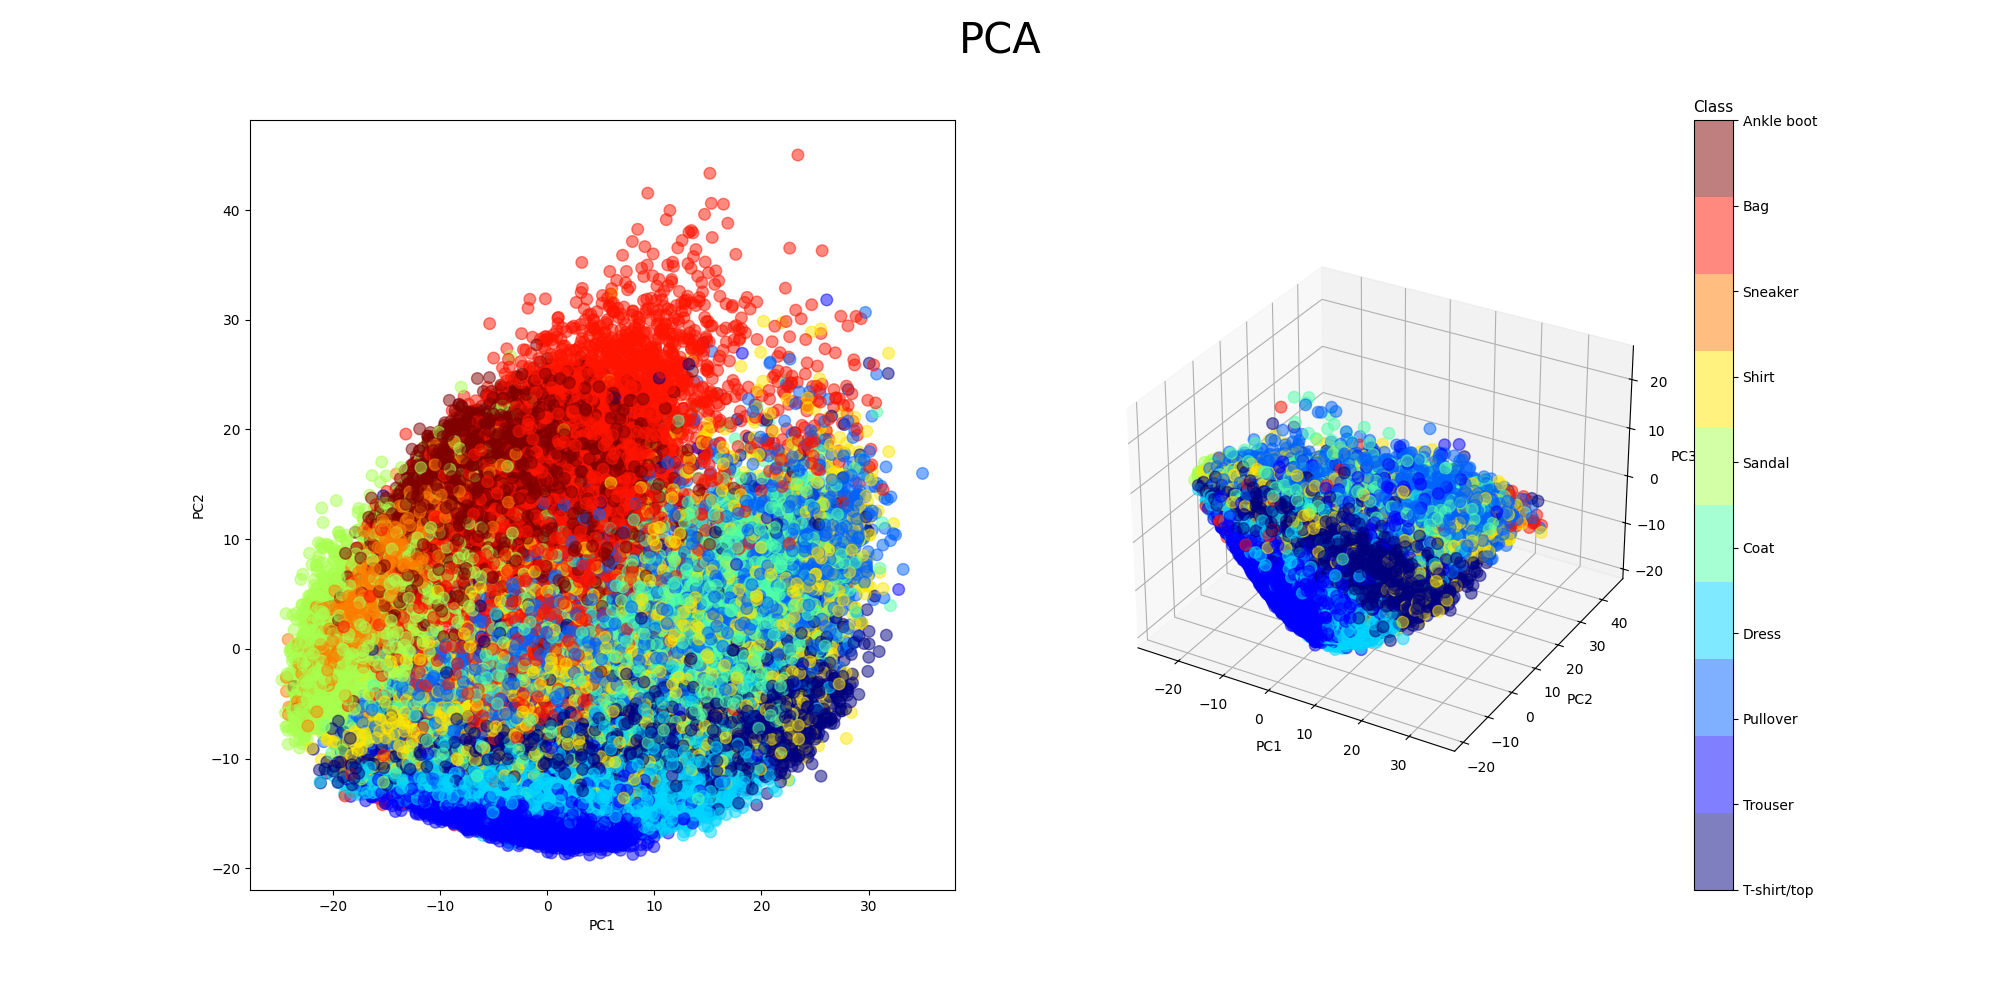
\includegraphics[width=0.8\textwidth]{images/pca.png}
    \caption{PCA visualization of the first two and three principal components.}
    \label{fig:pca}
\end{figure}

First I applied linear PCA to teh whole dataset and visualized the first two and three principal components.
The results are shown in Figure \ref{fig:pca}.

\subsection{Kernel PCA}
I then went on to apply Kernel PCA to the dataset, experimenting with different kernels and parameters using both 
RBF, polynomial and sigmoid kernels. The algorithm was applied to $\frac{1}{20}$-th of the dataset, due to computational
reasons, however the results are still meaningful.

\begin{figure}[ht]
    \centering
    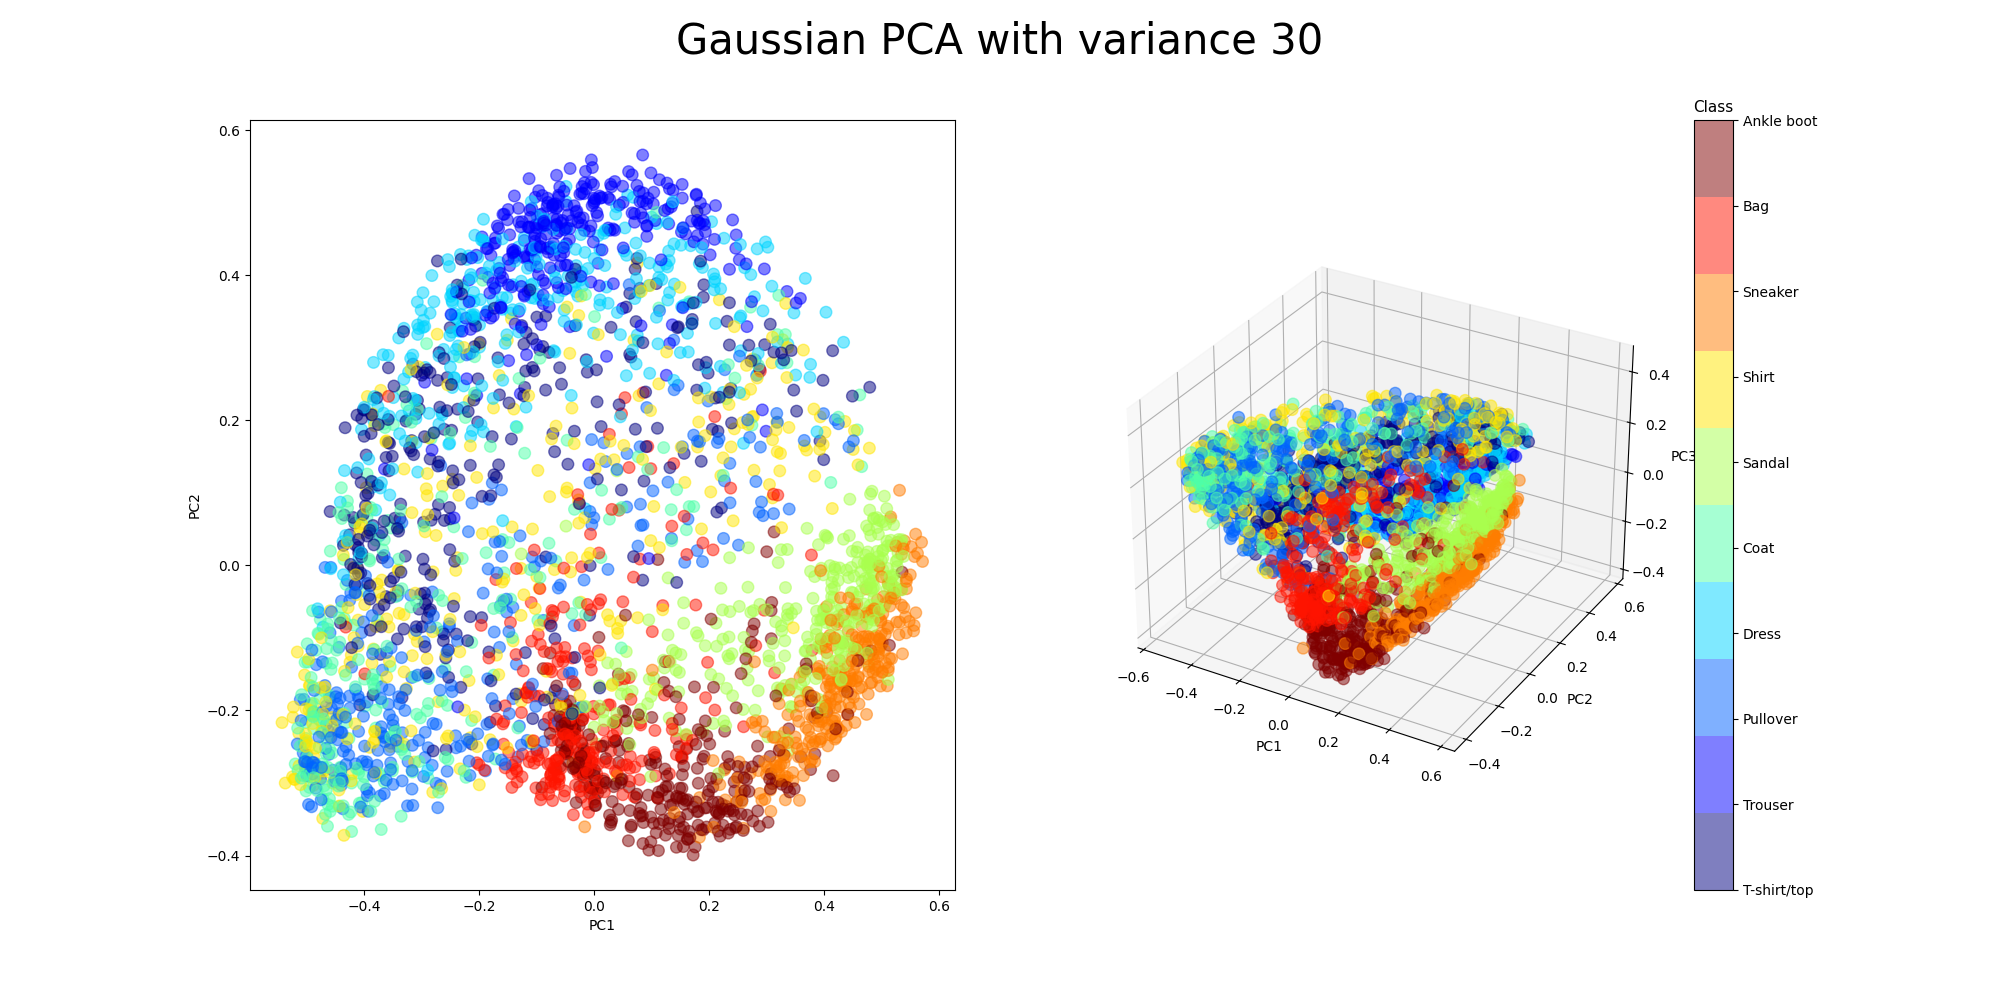
\includegraphics[width=0.8\textwidth]{images/kernel_pca.png}
    \caption{Kernel PCA visualization of the first two and three principal components.}
    \label{fig:kpca}
\end{figure}

The RBF kernel, with variance parameter $\sigma = 30$ provides the best separation, capturing the non-linear relationships 
between the data points without incurring in overfitting.
The results are shown in Figure \ref{fig:kpca}.

\section{\textit{Hybrid} Unsupervised - Supervised Approach}
\subsection{KMeans Clustering}
Then I proceeded to first reduce the dimensionality of the dataset using Kernel PCA with RBF kernel and $\sigma = 30$ on 10 components. As pictured in the
Figure \ref{fig:kpca_spectrum}, we can picture an elbow in the spectrum of the explained variance, which suggests that 10 components are enough, even though
the cumulative explained variance is not very high. This phenomenon is expectable, as we are trying to shrink the dataset from 784 to 10 dimensions.

\begin{figure}[ht]
    \centering
    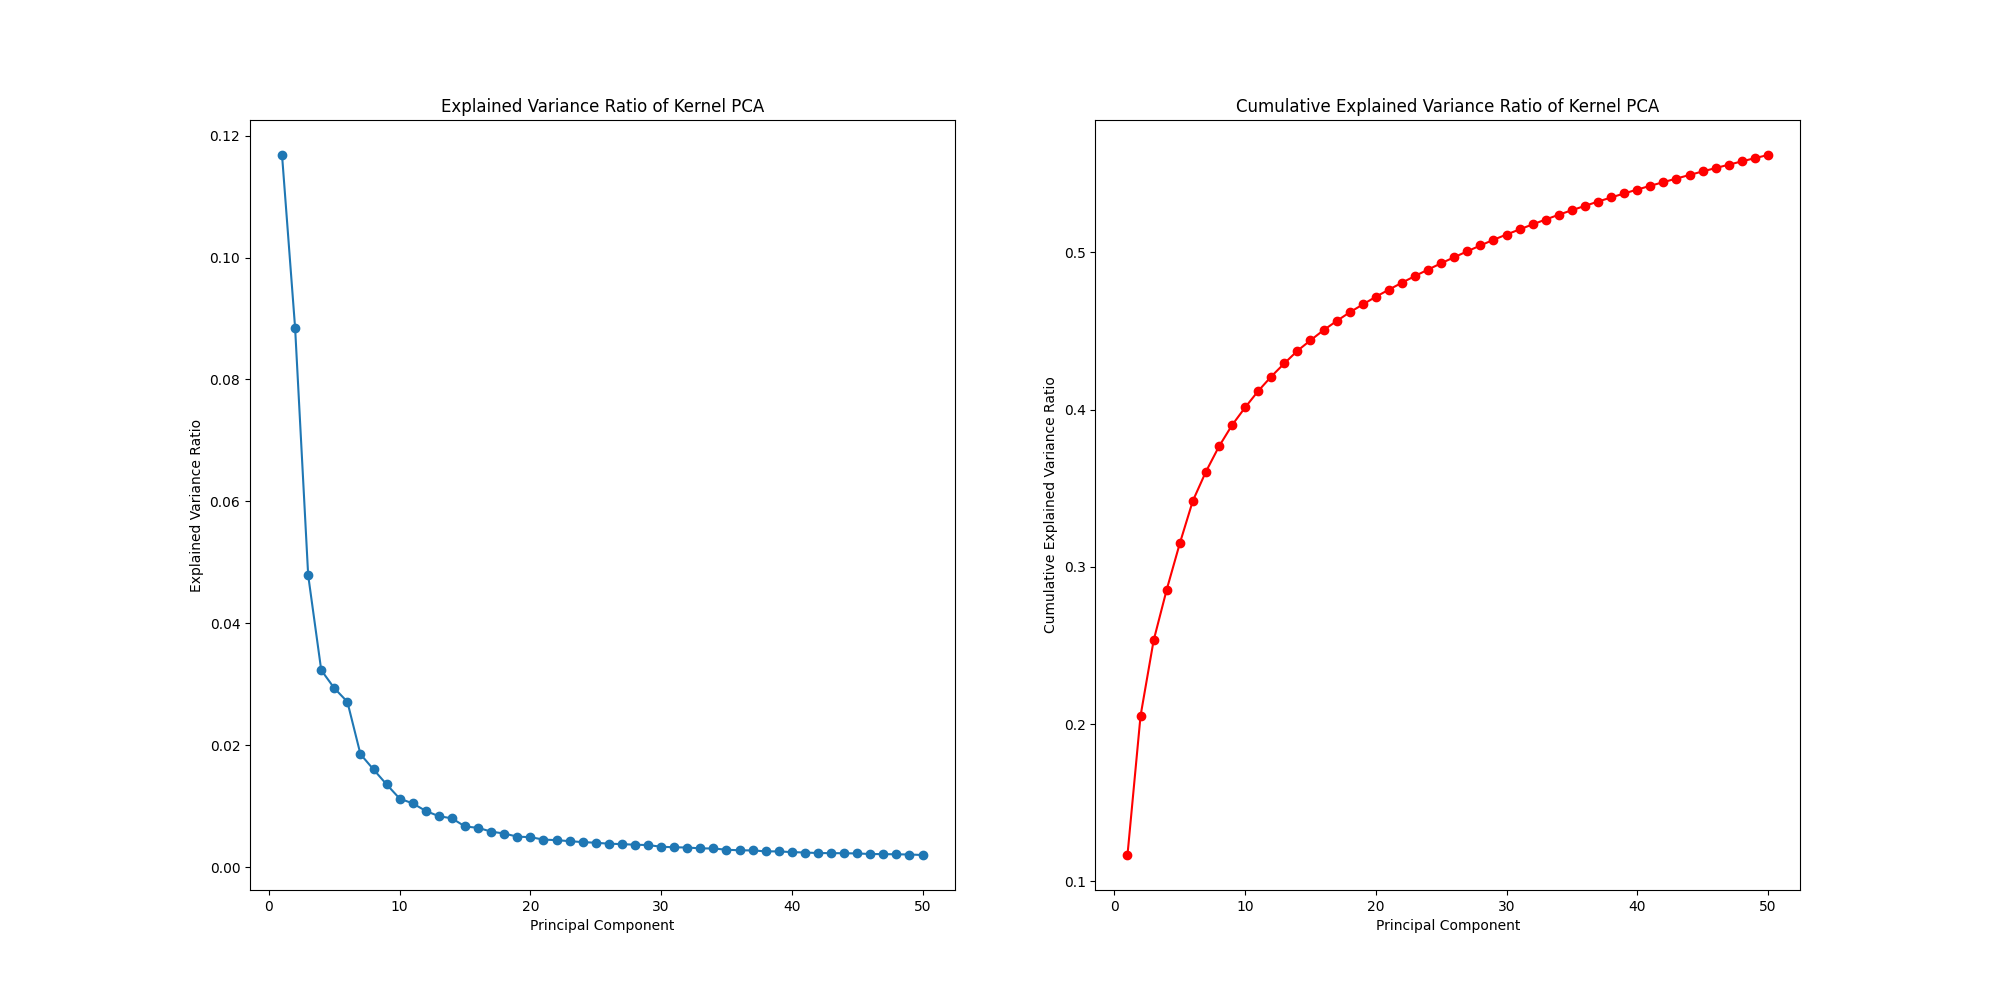
\includegraphics[width=0.8\textwidth]{images/kpca_spectrum.png}
    \caption{Explained variance spectrum of Kernel PCA with RBF kernel and $\sigma = 30$.}
    \label{fig:kpca_spectrum}
\end{figure}

Then I applied KMeans clustering to the reduced dataset, with $k = 10$ clusters, in order to see if the obtained clusters reflect the original label distribution.
The results are shown in Figure \ref{fig:kmeans}.
\begin{figure}[ht]
    \centering
    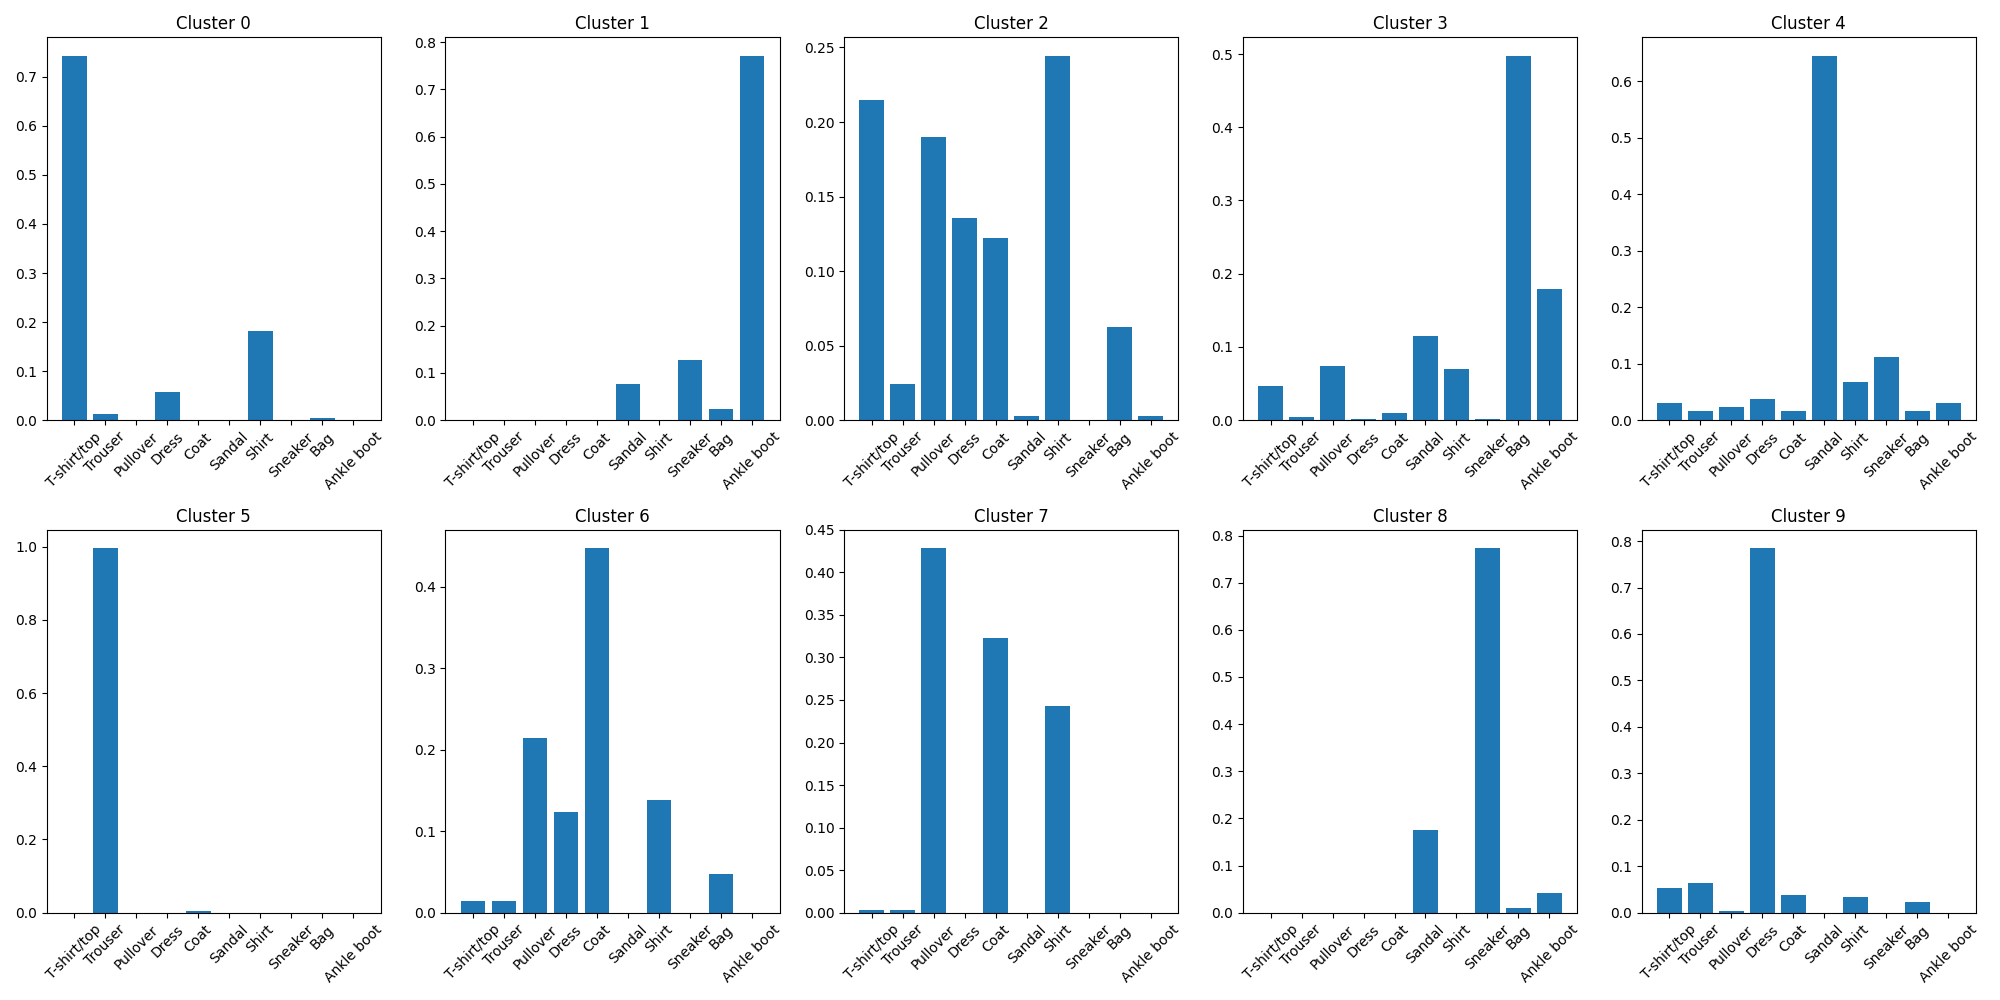
\includegraphics[width=0.8\textwidth]{images/kmeans.png}
    \caption{KMeans clustering of the reduced dataset.}
    \label{fig:kmeans}
\end{figure}
Looking at the label distribution in the clusters, we can see how most of them are composed of mainly one class, reflecting a good separation between classes.
However, some of them are characterized by a mixed distribution of about 2-3 classes, and mainly referred to upper-body clothes.

\subsection{Supervised Classification on Clusters}
Finally, I applied a supervised classification algorithm to the clusters obtained from the KMeans clustering. I used various models, such as kernel-SVM and Neural Networks.
In what follows, I will briefly recap the performances of the models trained. The best models were selected based on the validation accuracy.

\subsubsection{Kernel-SVM}
For this part I experimented with various kernels, such as RBF, polynomial and sigmoid, trying to perform also some hyper-parameter tuning.
\begin{itemize}
    \item Gaussian RBF Kernel:
        \subitem $\sigma = 10$ shows clear signs of overfitting, with a training accuracy of $1.0$ and a validation accuracy of $0.73$.
        \subitem \underline{Best Model}: $\sigma = 25$, with a training accuracy of $0.95$ and a validation accuracy of $0.93$.
    \item Polynomial Kernel:
        \subitem This kernel showed more consistent performance, both on training and validation accuracy.
        \subitem \underline{Best Model}: $d = 3$, with a training accuracy of $0.92$ and a validation accuracy of $0.92$.
    \item Sigmoid Kernel:
        \subitem This kernel showed the worst performance overall, with very poor validation accuracy.
        \subitem \underline{Best Model}: $\gamma = 0.01$, with a training accuracy of $0.41$ and a validation accuracy of $0.43$.
\end{itemize}
Overall, the best model resulted to be the one exploiting the Gaussian RBF kernel, with $\sigma = 25$, with both high training and validation accuracy, symptom
of a good generalization.

\subsubsection{Fully Connected Neural Networks}
I also experimented with fully connected neural networks, with different architectures and hyperparameters.

\begin{itemize}
    \item Smaller Neural Network:
        \subitem 128 hidden units for two layers, with ReLU activation function, 20 epochs and learning rate of $0.001$.
        \subitem Reached a training accuracy of $1.0$ and a validation accuracy of $0.92$.
        \subitem Shows signs of overfitting at later epochs.
    \item Bigger Neural Network:
        \subitem 256 hidden units for two layers, with ReLU activation function, 20 epochs and learning rate of $0.0005$.
        \subitem Reached a training accuracy of $1.0$ and a validation accuracy of $0.93$.
        \subitem Slight better gereralization roperties than the first network, but still shows signs of overfitting at later epochs.
\end{itemize}

\subsubsection{Convolutional Neural Networks}
Finally, I experimented with Convolutional Neural Networks, which are known to perform well on image classification tasks.

\begin{itemize}
    \item Achieved almost the best performance among the models trained, with a validation accuracy of $0.93$.
    \item Keeping the training accuracy lower than $1.0$, we can see that the model is able to generalize better.
    \item Showed lower signs of overfitting than the fully connected neural networks.
\end{itemize}

\subsubsection{Comparisons}
\begin{enumerate}
    \item Kernel-SVM outperformed all types of Neural Networks, with the best model reaching a validation accuracy of $0.94$.
    \item Among the neural networks, the Convolutional Neural Network showed the better generalization properties, likely to their ability to capture spatial
    relationships in the data.
    \item Both FCN showed signs of overfitting, above all when trained on higher number of epochs.
\end{enumerate}

These results suggest that the best model for classifying the clusters obtained from the KMeans clustering on reduced data is the kernel-SVM, maybe due to the 
fact that the clusters were constructed with kernel-reduced data on similar parameters. However, the Convolutional Neural Network results show that on further optimization
(even simply more data), they could match or even outperform the kernel-SVM.

High validation accuracies on cluster labels shows that clustering was able to capture the main underlying structure of the data. It is important to note, however,
that this classification is made on the clustering labels, not on the actual Fashion-MNIST labels, which can explain the strangely high accuracies in a dataset like this,
where the usual accuracies are around $0.9$.

\subsection{Performance on Test Set with real labels}
As final part of the pipeline, I tested the best model obtained on the test set, with the real labels. In order to conduct this test, I employed two methods: one
consisting in assigning as \textit{real label} of each cluster the most frequent label in the cluster (this approach is called \textit{Majority Voting}, which
could be mimicked by sampling some points from each cluster and manually assign the label related to the most frequent class), and another one more \textit{probabilistic} in
a fuzzy c-means fashion, where the label of a point is assigned sampling from the probability distribution of the labels in the cluster.

The resulted about class-wise and weighted accuracies are reported in the table below.
\begin{table}[ht]
    \centering
    \begin{tabular}{|c|c|c|c|c|}
        \hline
        \textbf{Class} & \textbf{SVM} & \textbf{FCN1} & \textbf{FCN2} & \textbf{CNN} \\
        \hline
        \hline
        T-shirt/top & 0.58 & 0.58 & 0.58 & 0.59 \\
        Trousers    & 0.91 & 0.90 & 0.90 & 0.90 \\
        Pullover    & 0.41 & 0.43 & 0.43 & 0.42 \\
        Dress       & 0.68 & 0.67 & 0.67 & 0.67 \\
        Coat        & 0.47 & 0.47 & 0.47 & 0.47 \\
        Sandal      & 0.55 & 0.52 & 0.52 & 0.53 \\
        Shirt       & 0.27 & 0.27 & 0.27 & 0.26 \\
        Sneaker     & 0.79 & 0.78 & 0.78 & 0.78 \\
        Bag         & 0.60 & 0.60 & 0.60 & 0.60 \\
        Ankle boot  & 0.72 & 0.71 & 0.71 & 0.71 \\
        \hline
        Accuracy    & 0.59 & 0.59 & 0.59 & 0.59 \\
        \hline
    \end{tabular}
    \caption{Class-wise and weighted accuracies on the test set using majority voting.}
    \label{tab:majority}
\end{table}

\begin{table}[ht]
    \centering
    \begin{tabular}{|c|c|c|c|c|}
        \hline
        \textbf{Class} & \textbf{SVM} & \textbf{FCN1} & \textbf{FCN2} & \textbf{CNN} \\
        \hline
        \hline
        T-shirt/top & 0.38 & 0.40 & 0.39 & 0.40 \\
        Trousers    & 0.84 & 0.83 & 0.83 & 0.83 \\
        Pullover    & 0.30 & 0.29 & 0.27 & 0.29 \\
        Dress       & 0.51 & 0.53 & 0.50 & 0.50 \\
        Coat        & 0.37 & 0.35 & 0.35 & 0.36 \\
        Sandal      & 0.33 & 0.33 & 0.36 & 0.33 \\
        Shirt       & 0.20 & 0.17 & 0.18 & 0.20 \\
        Sneaker     & 0.65 & 0.66 & 0.63 & 0.63 \\
        Bag         & 0.39 & 0.41 & 0.42 & 0.41 \\
        Ankle boot  & 0.58 & 0.59 & 0.58 & 0.58 \\
        \hline
        Accuracy    & 0.45 & 0.46 & 0.45 & 0.45 \\
        \hline
    \end{tabular}
    \caption{Class-wise and weighted accuracies on the test set using fuzzy assignment.}
    \label{tab:fuzzy}
\end{table}

Table \ref{tab:majority} shows the results using the majority voting method, while Table \ref{tab:fuzzy} shows the results of the test set evaluation 
using the fuzzy assignment method,. We can observe that the results are in both cases pretty low, reaching some consistent $60\%$ accuracy in the \textit{majority voting} 
scenario, while only about $45\%$ in the fuzzy assignment. This is due to the fact that the clusters obtained from the KMeans don't mirror exactly the original
labels, with more clusters showing mixed label distributions. This is reflected even more in the accuracy of the fuzzy assignment, as introducing a 
probabilistic assignment makes the model more sensible to the mixed distributions in the clusters.

However, we can see some interesting results regarding the class-wise accuracies: 
\begin{itemize}
    \item Trousers, Sneakers and Ankle boots are the classes with the highest accuracies, showing that the clusters obtained for these classes are \textit{cleaner},
    in the sense that they contain mainly points of the same class.
    \item Looking at the \textit{majority voting} accuracies, we have "high" accuracies also for the labels Dress and Bag.
    \item The class with the lowest accuracies are Shirt, Coat and Pullover, which are the classes with the most mixed distributions in the clusters. This behavior can be 
    explained by the fact that these classes are more similar to each other, so we expect that characterizing features lie in higher dimensions than the ones
    used for the clustering (10 dimensions representing about 40\% of the variance of the data).
\end{itemize}

This result highlights how the unsupervised-to-supervised pipeline captured some maningful structure in the data, reflected in the high validation accuracies, 
but there is a significant drop in performance when we pass to the original Fashion-MNIST labels. The consistent difficulty of the models to distinguish classes like
T-shirt/top and Shirt, or Coat and Pullover, shows how these classes were mixed during the clustering phase, maybe due to the fact that they share some features
in the reduced space. Maybe moving to a higher-dimensional space above all when using the kernel-PCA could help in capturing more complex relationships between
features and help in distinguishing these classes during clustering phase.

The significantly low performance of these models (45-60\% accuracy) on the test set on this type of dataset, compared to the usual accuracies classification 
accuracies on Fashion-MNIST (above 90\%), highlights significant challenges in the unsupervised-to-supervised pipeline, especially when dealing with mixed 
distributions in the clusters. However, the fact that all models perform well above random guessing (10\% accuracy) shows that the pipeline was able to capture
some meaningful structure in the data.

\section{Fully Supervised Approach}

As last step, I performed the classification approach in a fully supervised framework, so using the true label assignment during training.

\subsection{Model Performance}
I trained the same models used in the previous section, but this time using the true labels for training. The results are shown in the table below.

\begin{table}[ht]
    \centering
    \begin{tabular}{|c|c|c|}
        \hline
        \textbf{Model} & \textbf{Hybrid pipeline (fuzzy assignment)} & \textbf{Fully supervised} \\
        \hline
        \hline
        SVM  & 0.45 & 0.81 \\
        FCN1 & 0.46 & 0.55 \\
        FCN2 & 0.45 & 0.59 \\
        CNN  & 0.45 & 0.66 \\
        \hline
    \end{tabular}
    \caption{Comparison of the models' performance in the hybrid and fully supervised pipeline.}
    \label{tab:comparison}
\end{table}

\subsection{Class-wise Accuracies}
The class-wise accuracies of the models trained in the fully supervised pipeline are by far higher than the ones obtained in the hybrid pipeline, showing a 
consistent value above $60\%$ for almost all classes, but again the classes Shirt, Coat and Pullover show the lowest accuracies, of around 40\%.

This result highlights how the fully supervised approach is able to capture more complex relationships between features and labels, and is able to distinguish
more easily between classes that are more similar to each other.

\subsection{Trial of Neural Networks on not-scaled data}
As a last attempt, I tried to train the Neural Networks on the not-scaled data, in order to see how the models are able to deal with the scaling of the data.
The results are shown in the table below.

\begin{table}[ht]
    \centering
    \begin{tabular}{|c|c|c|}
        \hline
        \textbf{Model} & \textbf{Scaled data} & \textbf{Not-scaled data} \\
        \hline
        \hline
        SVM  & 0.81 &  -   \\
        FCN1 & 0.55 & 0.81 \\
        FCN2 & 0.59 & 0.81 \\
        CNN  & 0.66 & 0.86 \\
        \hline
    \end{tabular}
    \caption{Comparison of the models' performance on scaled and not-scaled data.}
    \label{tab:scaling}
\end{table}

The results show that the Neural Networks are able to deal autonomously with the scaling of the data, by learning the proper one.
In this framework we can see how the Fully Connected Neural Networks are able to perform as the SVM, while the Convolutional Neural Network is able to perform
even better, reaching an accuracy of $0.86$ on the not-scaled data.

\section{Discussion}

\subsection{Dimensionality Reduction and Clustering}
The PCA and Kernel-PCA highlighted the complex non linear relations in the Fashion-MNIST dataset. The k-Means clustering on the reduced data was able to capture
some meningful insights in the data, as showed by the distribution of labels in each cluster. However exploiting only these few dimensions (10) for clustering
resulted to be not enough to capture the full complexity of the data, as showed by the repetition of the most frequent label per cluster, and the presence of 
mixed distributions in some clusters.

\subsection{Hybrid vs. Supervised Classification}
The hybrid pipeline showed some interesting results, demonstrating some potential in employing some preliminary unsupervised learning techniques to create a
rudimental \textit{baseline} classification system. However, the substantial performance gap with respect to the fully supervised approach (of about 10-40\%) shows how the
importance of label assignment in this task. 

Moreover, the performance gap of the NNs on the not-scaled data, compared to the scaled data, shows how powerful the Neural Networks are in not only capturing
the meaningful structure in the data, but also in dealing with the proper transformations.

\subsection{Model Comparison}
Unexpectedly, applying the kernel-SVM and the NNs on the same data, showed how in principle simpler models like the kernel-SVM are able to outperform the NNs,
outlining how the decision boundaries on this kind of data can be easily captured by SVM's kernel trick. However, we can see how, feeding the Neural Networks 
with not scaled data we are able to reach better performances, even on a small amount of data.

\section{Conclusions}
This challenge showed how we can deep-dive into Kernel methods and Neural Networks using only a toy dataset like Fashion-MNIST. The results showed, expectedly,
how a fully-supervised approach performs by far better than a hybrid unsupervised-to-supervised pipeline, but how the latter is able to provide some meaningful 
insights in the data structure. Moreover, seeing how SVMs are able to perform almost equally to fully connected Neural Networks in this image classification task
shows how powerful the kernel trick can be in capturing complex relationships in the data, above all when dealing with small datasets.

\end{document}